\documentclass[border=8pt]{standalone}
\usepackage{tikz}
\usetikzlibrary{arrows.meta,positioning,calc}
\begin{document}
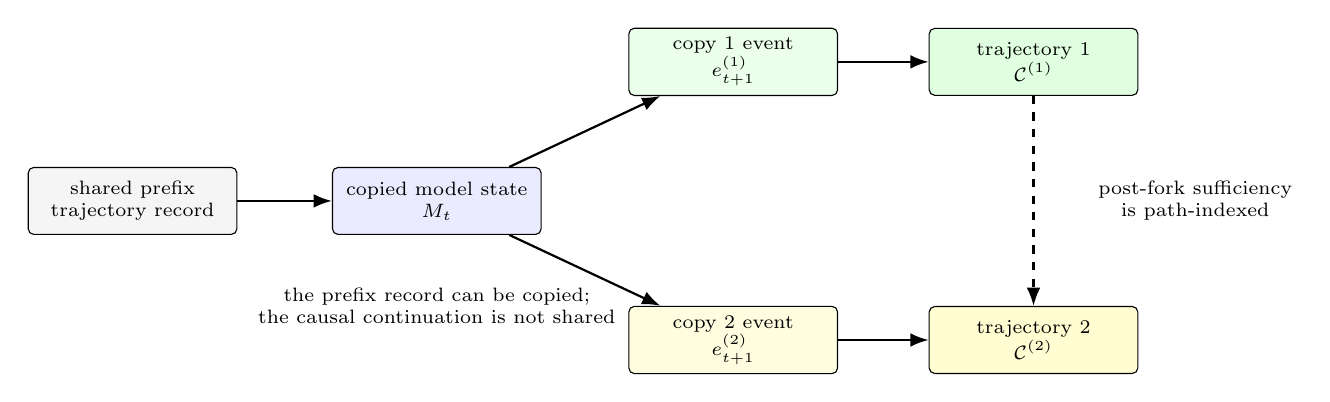
\begin{tikzpicture}[
  box/.style={draw, rounded corners=2pt, align=center, minimum width=2.65cm, minimum height=0.85cm, font=\scriptsize},
  note/.style={align=center, font=\scriptsize},
  arr/.style={-Latex, thick},
  dasharr/.style={-Latex, thick, dashed}
]

\node[box, fill=gray!8] (prefix) {shared prefix\\trajectory record};
\node[box, fill=blue!8, right=1.2cm of prefix] (copy) {copied model state\\$M_t$};
\draw[arr] (prefix) -- (copy);

\node[box, fill=green!8, above right=0.9cm and 1.1cm of copy] (a1) {copy 1 event\\$e_{t+1}^{(1)}$};
\node[box, fill=yellow!12, below right=0.9cm and 1.1cm of copy] (a2) {copy 2 event\\$e_{t+1}^{(2)}$};
\draw[arr] (copy) -- (a1);
\draw[arr] (copy) -- (a2);

\node[box, fill=green!12, right=1.15cm of a1] (c1) {trajectory 1\\$\mathcal C^{(1)}$};
\node[box, fill=yellow!18, right=1.15cm of a2] (c2) {trajectory 2\\$\mathcal C^{(2)}$};
\draw[arr] (a1) -- (c1);
\draw[arr] (a2) -- (c2);

\node[note, right=0.7cm of $(c1)!0.5!(c2)$] {post-fork sufficiency\\is path-indexed};
\draw[dasharr] (c1) -- (c2);
\node[note, below=0.55cm of copy] {the prefix record can be copied;\\the causal continuation is not shared};

\end{tikzpicture}
\end{document}
